%##############################################################################
% Preamble
%##############################################################################

\documentclass{pset}
\name{Dustin Tran, Xiaomin Wang, Rodrigo Gomes}
\email{\{trandv,xiaominw, rgomes\}@mit.edu}

\course{6.834J/16.412J, S15}
\instructor{Professor Brian Williams}
\assignment{Problem Set \#3}
\duedate{April 17, 2015}

\begin{document}

%##############################################################################
% Begin Document
%##############################################################################

\section{Introduction}
Natural scenarios in real life occur where one must sequentially make decisions
under uncertainty. Quite often not only are transitions to certain states
unknown but the true state of the agent as well. This is similar to that of a
hidden Markov model (HMM), only in that one must make a sequence of actions
instead of a single action. The classic scenario is a robot navigating a
discrete environment using a GPS, and it takes action that lead to different
states with various probabilities, but because of the GPS there is also
inaccuracy in what its current state is.

One can formalize this, under Markovian assumptions, as a partially observable
Markov decision process (POMDP). In this project we provide a software
library for solving them with modular classes in order to allow for flexible
extensions.  More specifically, we encode a variety of basic tasks and solve
them using a combination of value iteration and a variant of Thompson sampling 
\cite{strens2000bayesian}, which is a Bayesian approach
following a Dirichlet-multinomial posterior over each state-action pair. 

\section{Technical Background}

\subsection{POMDP}
POMDP is a generalization of a Markov decision process (MDP). In an MDP, for each possible state of
the process, a decision has to be made regarding which action should be executed in that state. The
chosen action affects both the transition probabilities and the costs (or rewards) incurred. The
goal is to choose an optimal action in every state to increase some predefined measure of 
performance. In a POMDP model, the agent cannot fully observe the system states. 
Instead, it must maintain a probability distribution over the set of possible states, 
based on a set of observations and observation probabilities, and the underlying MDP.  

More formally, a POMDP is represented by the following variables: 

\begin{itemize}
\item $S$ is a set of states
\item $A$ is a set of actions
\item $T$ is a set of transition probabilities between states. If the agent is currently in state $s
\in S$, and it takes action $a \in A$. The agent will transition to some new state $s'$ according to 
$T(s' \mid s,a)$
\item $R: S \times A \rightarrow \mathbb{R}$ is a reward function that assigns a numeric reward (or
cost if the value is negative) for each state and action. 
\item $\Omega$ is a set of observations
\item $O$ is a set of conditional observation probabilites. If the agent is now in state $s$, 
it receives an observation $o$ according to $O(o \mid s)$
\item $\gamma \in [0,1]$ is a discount factor that determines how much rewards should be discounted over time
\end{itemize}
 
We use our testing environment, gridworld, as an example. 
Gridworld represents a 2D maze where the agent can be in discrete locations. Certain
locations are impossible for the agent, representing ``walls''. Every action can
move the agent between two adjacent grid locations, or fail, and keep the agent in
the same location with some probability. The objective is to reach the goal location. 
For the gridworld, $S$ consists of all the possible (row, column) location tuples inside the maze. 
$A$ contains the four possible actions the agent can take: up, down, left, right. 
$T$ describes a transition model that allows the agent to move without hitting the wall. 
We define $R$ as: the agent has negative reward for every state/action, except when it reaches a goal state, 
where it has a high positive reward.
We implemented two observation models. The easier model gives the agent more information about the
environment. The agent knows which of its four neighbors are walls, giving rise to 16 total
observations. In the other observation model, the agent can only observe how many of its four
neighbors are walls, giving rise to 5 possible observations. $O$ is such that 
$Pr(true\_observation\mid state)=true\_observation\_prob$, where $true\_observation\_prob$ can be adjusted.
And $Pr(other\_observation\mid state)=\frac{1-true\_observation\_prob}{total\_num\_of\_observations-1}$
Since we cannot work with the underlying states directly in POMDP, we also need $B$ which is the set
of belief states, or the probabilities the agent is at all possible states. 

\subsection{Value Iteration}
We solve POMDP with value iteration. Value $V$, is the expected total reward
given a policy $\pi$, where a policy decides which action to take given the belief state. $a =
\pi(b)$. The expected reward for policy $\pi$ starting freom belief $b_0$ is defined as 
\[ V^{\pi}(b_{0})=\sum\limits_{t=0}^\infty \gamma^{t}r(b_t,a_t) \]
where $r(b_t, a_t) = \sum\limits_{s \in S} b_t(s)R(s,a_t)$.

The optimal policy should maximize the long term reward
\[ \pi = \underset{\pi}{\text{argmax}} V^{\pi}(b_0) \]
At each time step, we update the belief states based on the observation, and then update the values based on
the updated belief states. The action that gives the largest expected reward over the belief states
is selected for the next time step. The updating algorithm is a form of Thompson Sampling, which
will be introduced in the next section. The values gradually improve until convergence. By improving the values,
the policy is implicitly improved. 

\subsection{Thompson Sampling}
Thompson Sampling is used to learn the transition model and to select the best action.
The transition model, $T$ is initialized uniformly. After every some number of  time steps (samples), 
the transition probabilities are recalculated using Bayesian methods. In MDP, since the agent can observe the states
directly, the posterior transition probabilities are updated using the transition counts.
In POMDP, the posterior probabilities are updated using belief state transition probabilities. 
Every few steps, the value table is also updated.


\section{Implementation}
For use with POMDPs, we assume that the agent is given an observation model of the
environment it is acting in, in the form of a conditional probability distribution
$P(observation \mid state)$. Astrom has shown that a properly updated probability 
distribution over the state space S is sufficient to summarize all the observable 
history of a POMDP agent without loss of optimality \cite{astrom}. The agent, however, is unaware of its transition model, and
reward model, and must learn those. Using these models, the agent keeps, and
updates a distribution over the states it can be in, and chooses the action with
the highest expected reward.


\subsection{Agent Environment Paradigm}

\subsection{Organization of Code}
We follow the directory structure specified in the problem set, with two
exceptions:
\begin{itemize}
\item \texttt{documentation/} does not exist. Instead, documentation is written
in the \texttt{README.md} inside the current working directory. Any additional
documentation not purely necessary for the problem set submission is in the
Github wiki.
\item \texttt{source/} is named \texttt{bayesrl/} in order to follow Python
convention for installing modules.
\end{itemize}

\section{Analysis}

\subsection{Runtime}

\subsection{Memory}

\subsection{Limitations}

\section{Benchmark Results}
The implementation of Thompson Sampling for MDPs ran very successfully: as time
progressed, the agent was able to get to the goal much faster, and get a high
reward. It did not work, however, for POMDPs. As time progressed, the agent seemed
to take about the same amount of time to reach the goal on every execution, not
improving in performance. We hypothesize that the reason is due to a lack of
a good prior on the transition model: thompson sampling relies a lot on being
able to count the number of transitions between states, given an action. This
is very hard in a POMDP with a weak prior on its transition model, as it may have
a completely wrong idea of where it ends up at each step. The observation model
is supposed to improve its accuracy, but it was not sufficient in this case.

To have an idea of how differently successful the same approach was on MDPs vs
POMDPs, we show you our results:

\begin{figure}
\centering
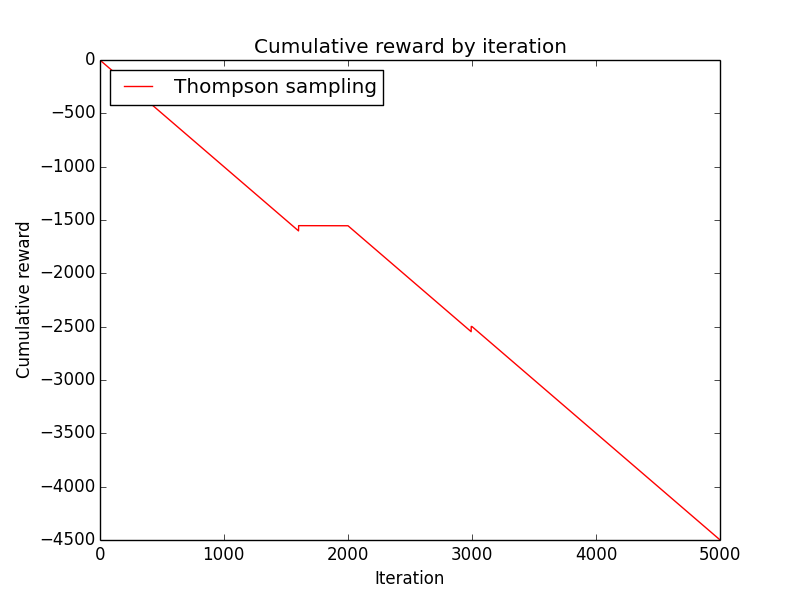
\includegraphics[width=0.5\textwidth]{pomdp.png}
\caption{\label{fig:pomdp}Cumulative Reward for POMDP}
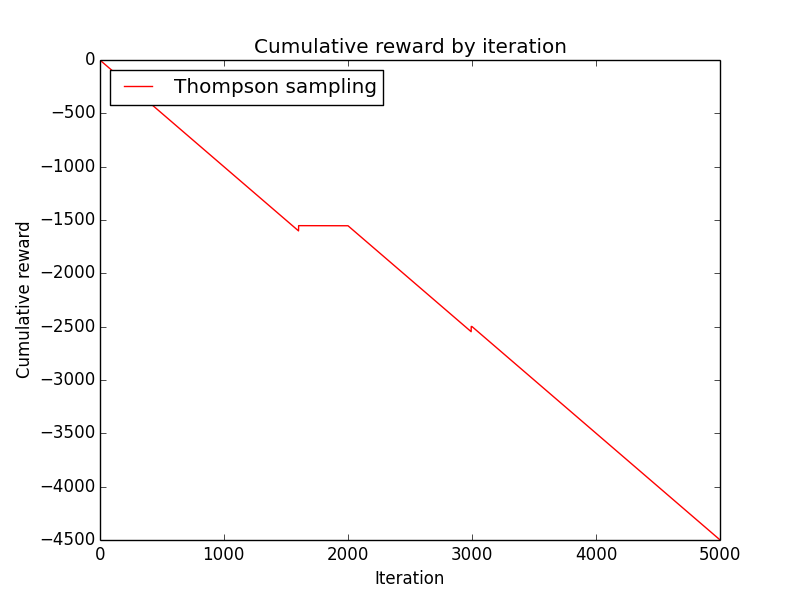
\includegraphics[width=0.5\textwidth]{pomdp.png}
\caption{\label{fig:mdp}Cumulative Reward for MDP}
\end{figure}

These graphs show the cumulative reward that the agent got as time progressed.
In the MDP case, the reward started low, and kept getting lower, as the agent
explored. It, however, started getting higher as the agent started acting in a
more deliberate manner, to maximize reward. The POMDP agent, however, seems to
be in a state where its reward just gets increasingly negative. It is unclear
whether it never leaves the exploration phase, or if it simply learns a completely
wrong transition model, and thus computes a very wrong policy.



\bibliography{6_834j_ps03}
\bibliographystyle{plain}

%##############################################################################
% End Document
%##############################################################################

\end{document}
